\documentclass[a4paper,12pt,oneside,openany]{book}

% ============================================================================
% PROJETO FINAL - BANCO DE DADOS I
% UNESP - Faculdade de Ciencias - Departamento de Computacao
%
% COMO USAR:
% 1) O Capitulo 1 (Modelagem Conceitual) esta COMPLETO. Ele fixa o vocabulario
%    do projeto: nomes de entidades, de atributos e de tabelas. Os capitulos
%    seguintes devem respeitar exatamente esses nomes.
% 2) Os Capitulos 2 e 3 sao esqueletos. Cada secao traz uma \orientacao
%    explicando o que se espera ali e, quando possivel, a tabela ja montada
%    para ser preenchida.
% 3) Todo diagrama precisa de explicacao no texto. Diagrama sem prosa nao
%    comunica decisao de projeto.
% 4) Toda decisao relevante (por que especializacao e nao tabela unica, por
%    que gatilho e nao CHECK) deve ser justificada por escrito.
% 5) Antes da entrega, troquem \orientacoestrue por \orientacoesfalse: as
%    orientacoes e o apendice de divisao de trabalho somem do PDF.
% ============================================================================

\usepackage[T1]{fontenc}
\usepackage[utf8]{inputenc}
\usepackage[brazil]{babel}
\usepackage{amsmath}
\usepackage{graphicx}
\usepackage{xcolor}
\usepackage{float}      % permite [H]: fixa o float exatamente onde ele esta
\usepackage{placeins}
\usepackage{booktabs}
\usepackage{tabularx}
\usepackage{longtable}
\usepackage{array}
\usepackage{enumitem}
\usepackage{hyperref}
\usepackage{fancyhdr}
\usepackage[top=2cm,bottom=2cm,left=2cm,right=2cm]{geometry}
\usepackage{listings}
\usepackage{needspace}

\definecolor{sqlkeyword}{HTML}{0B5394}
\definecolor{sqlcomment}{HTML}{6A737D}
\definecolor{sqlstring}{HTML}{A31515}

% ----------------------------------------------------------------------------
% Estilo para trechos de codigo SQL
% ----------------------------------------------------------------------------
\lstset{
    basicstyle=\ttfamily\footnotesize,
    breaklines=true,
    columns=fullflexible,
    keepspaces=true,
    showstringspaces=false,
    frame=single,
    rulecolor=\color{gray!40},
    captionpos=b,
    xleftmargin=1em,
    aboveskip=1em,
    belowskip=1em,
    extendedchars=true,
    literate=%
        {á}{{\'a}}1 {à}{{\`a}}1 {â}{{\^a}}1 {ã}{{\~a}}1
        {é}{{\'e}}1 {ê}{{\^e}}1 {í}{{\'i}}1 {ó}{{\'o}}1
        {ô}{{\^o}}1 {õ}{{\~o}}1 {ú}{{\'u}}1 {ü}{{\"u}}1
        {ç}{{\c c}}1 {Á}{{\'A}}1 {É}{{\'E}}1 {Ç}{{\c C}}1,
}

\lstdefinestyle{sql}{
    language=SQL,
    morekeywords={SERIAL, BOOLEAN, TIMESTAMP, NUMERIC, SMALLINT, TEXT, VARCHAR,
        RETURNS, TRIGGER, PLPGSQL, LANGUAGE, EXECUTE, FUNCTION, RETURN, IF,
        THEN, RAISE, EXCEPTION, NEW, OLD, BEFORE, AFTER, EACH, ROW, SCHEMA,
        CASCADE, RESTRICT, SEARCH_PATH, REPLACE, MATERIALIZED},
    keywordstyle=\color{sqlkeyword}\bfseries,
    commentstyle=\color{sqlcomment}\itshape,
    stringstyle=\color{sqlstring},
}

\lstset{style=sql}

% Folga extra para nomes longos em \texttt nao estourarem a margem.
\setlength{\emergencystretch}{3em}

\hypersetup{
    hidelinks,
    pdftitle={Sistema de Acompanhamento e Avaliação de Séries de TV -- Projeto de Banco de Dados},
    pdfauthor={Igor dos Reis Gomes}
}

\urlstyle{same}

% ----------------------------------------------------------------------------
% Exibicao das orientacoes do modelo
% ----------------------------------------------------------------------------
% Troquem para \orientacoesfalse antes de gerar a versao final para entrega.
\newif\iforientacoes
\orientacoestrue

\newcommand{\orientacao}[1]{%
    \iforientacoes
        \begin{quote}
        \small\itshape\textbf{Orientação:} #1
        \end{quote}
    \fi
}

% Atalho para identificadores do banco (tabelas, colunas, tipos).
\newcommand{\id}[1]{\texttt{#1}}

% ----------------------------------------------------------------------------
% Cabecalho e rodape
% ----------------------------------------------------------------------------
\renewcommand{\headrulewidth}{0pt}
\fancyhf{}

% ----------------------------------------------------------------------------
% Informacoes do trabalho -- CONFERIR ANTES DA ENTREGA
% ----------------------------------------------------------------------------
\newcommand{\school}{Universidade Estadual Paulista ``Júlio de Mesquita Filho'' (UNESP)\\
Faculdade de Ciências -- Bauru\\
Departamento de Computação}
\newcommand{\discipline}{Banco de Dados I}
\newcommand{\projtitle}{Sistema de Acompanhamento\\e Avaliação de Séries de TV}
\newcommand{\projsubtitle}{Modelagem conceitual, lógica e física de um banco de dados relacional}
\newcommand{\semester}{2026}

% ----------------------------------------------------------------------------
% Colocacao de floats
% ----------------------------------------------------------------------------
\renewcommand{\topfraction}{0.9}
\renewcommand{\bottomfraction}{0.7}
\renewcommand{\textfraction}{0.1}
\renewcommand{\floatpagefraction}{0.75}
\setcounter{topnumber}{3}
\setcounter{bottomnumber}{2}
\setcounter{totalnumber}{5}

\graphicspath{{images/}}

\title{Sistema de Acompanhamento e Avaliação de Séries de TV}
\author{Igor dos Reis Gomes}

\begin{document}

% ============================================================================
% CAPA
% ============================================================================
\thispagestyle{empty}
\begin{titlepage}
	\centering

	% Logotipo da UNESP no topo da pagina
	\vspace*{-12mm}
	
\includegraphics[width=75mm]{AV01A.jpg}\\[8mm]

	{\large\textbf{\school}}

	\vfill

	{\huge\textbf{\projtitle}}\\[5mm]
	{\Large\projsubtitle}

	\vfill

	{\Large\textbf{\discipline}}\\[14mm]

	% ATENCAO: conferir os integrantes do grupo de Banco de Dados I.
	Igor dos Reis Gomes -- RA: 241025265\\[2mm]
	\textit{Nome do segundo integrante} -- RA: \textit{000000000}\\[2mm]
	\textit{Nome do terceiro integrante} -- RA: \textit{000000000}\\[2mm]
	\textit{Nome do quarto integrante} -- RA: \textit{000000000}

	\vfill

	{\large Bauru -- SP\\\semester}
\end{titlepage}

\tableofcontents
\thispagestyle{empty}

\clearpage
\pagestyle{fancy}
\cfoot{\thepage}
\setcounter{page}{1}

\iforientacoes
\chapter*{Como utilizar este documento}
\addcontentsline{toc}{chapter}{Como utilizar este documento}

Este arquivo já contém a \textbf{modelagem conceitual completa} (Capítulo~\ref{cap:conceitual}).
Os Capítulos~\ref{cap:logica} e~\ref{cap:fisica} estão estruturados, mas precisam ser
escritos pelos demais integrantes.

O Capítulo~\ref{cap:conceitual} não é apenas a primeira etapa do trabalho: ele
\textbf{fixa o vocabulário} do projeto. Os nomes de entidades, atributos, tabelas e
colunas definidos ali valem para todo o restante do documento e para o script SQL.
Se alguma etapa posterior precisar alterar um nome, a alteração deve ser feita
\emph{também} no Capítulo~\ref{cap:conceitual}, para que o documento não se contradiga --
um esquema físico que não corresponde ao diagrama conceitual é o erro mais comum e mais
caro deste tipo de trabalho.

Os trechos marcados como \textit{Orientação} explicam o que se espera em cada seção.
Eles podem ser ocultados alterando-se, no início do arquivo,
\verb|\orientacoestrue| para \verb|\orientacoesfalse|. O Apêndice de divisão de
trabalho também desaparece nesse caso, pois é material interno do grupo.

\clearpage
\fi

% ============================================================================
\chapter{Modelagem Conceitual}\label{cap:conceitual}
% ============================================================================

Este capítulo descreve o minimundo escolhido pelo grupo, enuncia as regras de
negócio que o banco de dados deve sustentar e apresenta o diagrama
entidade-relacionamento (DER) correspondente.

O domínio foi escolhido por concentrar, em um cenário familiar a qualquer usuário,
as construções que a modelagem conceitual precisa exercitar: uma hierarquia de
composição em três níveis, relacionamentos muitos-para-muitos com atributos
próprios, um grafo social que relaciona um conjunto de entidades a ele mesmo e um
ato -- o de avaliar -- que incide indistintamente sobre três tipos de alvo.
Nenhuma dessas construções foi introduzida artificialmente para satisfazer o
enunciado: todas decorrem da forma como aplicações de acompanhamento de séries
efetivamente funcionam.

\section{Descrição do minimundo}

O sistema modelado é uma rede social voltada ao acompanhamento e à avaliação de
séries de televisão. Ele não exibe conteúdo audiovisual: registra e organiza o que
as pessoas assistem e o que elas acham do que assistiram. O paralelo mais próximo
são as plataformas de catalogação de filmes e de livros, como Letterboxd e Goodreads,
transposto para o formato seriado -- no qual a obra se subdivide em unidades menores, 
e cada uma dessas unidades pode ser assistida e avaliada separadamente.

O acervo do sistema é composto por \textbf{séries}, cada uma organizada em
\textbf{temporadas}, que por sua vez se dividem em \textbf{episódios}. Essa
hierarquia de três níveis é a espinha dorsal do minimundo, porque quase toda
interação do usuário acontece em um desses três níveis. Cada série é classificada
em um ou mais \textbf{gêneros} e conta com a participação de \textbf{pessoas} do
meio audiovisual, que podem atuar como atores, diretores, roteiristas ou criadores.
Uma mesma pessoa pode exercer funções diferentes em séries diferentes -- e até na
mesma série.

Os \textbf{usuários} do sistema mantêm uma relação individual com cada série do
acervo. Essa relação tem duas faces complementares. A primeira é a
\textbf{intenção declarada}: o usuário marca a série como algo que pretende
assistir, que está assistindo ou que abandonou. A segunda é o \textbf{histórico
efetivo}: o usuário registra, episódio a episódio, o que de fato assistiu e em que
data. As duas faces não são redundantes. Uma série pode estar marcada como
``pretendo assistir'' sem nenhum episódio registrado, e o progresso real de quem
está assistindo só pode ser calculado a partir dos registros individuais.

Sobre qualquer um dos três níveis da hierarquia, o usuário pode publicar uma
\textbf{avaliação}: uma nota, um texto crítico, ou ambos. Avaliar uma série
inteira, uma temporada específica ou um episódio isolado são atos de natureza
idêntica -- mudam apenas o alvo e o grau de detalhe -- e por isso são tratados no
modelo como um único conceito especializado em três formas.

A camada social se organiza em torno dessas avaliações. Um usuário pode
\textbf{seguir} outros usuários, o que constitui seu acompanhamento de atividade;
pode \textbf{curtir} avaliações alheias; e pode \textbf{comentar} nelas, inclusive
respondendo a comentários de outras pessoas. É importante notar que a curtida e o
comentário não incidem sobre a série nem sobre o autor isoladamente: eles incidem
sobre o \emph{ato de avaliar}, isto é, sobre a associação entre um usuário e um
item do acervo.

O minimundo organiza-se, portanto, em três pilares: o \textbf{acervo} (o dado
sobre a obra), o \textbf{acompanhamento} (a relação entre usuário e obra) e o
\textbf{social} (a relação entre usuários, mediada por avaliações).

\section{Regras de negócio}\label{sec:regras}

\orientacao{Cada regra abaixo precisa ser rastreável até uma construção concreta
do banco. Ao escrever os Capítulos~\ref{cap:logica} e~\ref{cap:fisica}, citem o
código da regra (RN01, RN02, \dots) ao lado da restrição, do gatilho ou da chave
que a implementa. A Seção~\ref{sec:rastreabilidade} traz a tabela de
rastreabilidade a ser preenchida.}

\paragraph{Usuários e relação social}
\begin{description}[leftmargin=2.2cm,style=nextline,font=\normalfont\bfseries]
    \item[RN01] Cada usuário é identificado por um \id{username} único no sistema,
    composto apenas por letras minúsculas, dígitos e sublinhado, com 3 a 30
    caracteres. O endereço de e-mail também é único.
    \item[RN02] Um usuário pode seguir outros usuários. A relação é
    \textbf{unidirecional}: seguir alguém não implica ser seguido de volta.
    \item[RN03] Nenhum usuário pode seguir a si mesmo.
    \item[RN04] A exclusão de um usuário implica a exclusão de todo o seu
    histórico: estados declarados, registros de exibição, avaliações, curtidas e
    comentários.
\end{description}

\paragraph{Acervo}
\begin{description}[leftmargin=2.2cm,style=nextline,font=\normalfont\bfseries]
    \item[RN05] Toda série pertence a pelo menos um gênero e pode pertencer a
    vários.
    \item[RN06] Toda temporada pertence a exatamente uma série, e seu número é
    único \emph{dentro} daquela série. Não existe temporada fora de uma série.
    \item[RN07] Todo episódio pertence a exatamente uma temporada, e seu número é
    único \emph{dentro} daquela temporada. Não existe episódio fora de uma
    temporada.
    \item[RN08] A exclusão de uma série implica a exclusão de suas temporadas e,
    por consequência, de seus episódios.
    \item[RN09] Uma pessoa pode participar de várias séries, e em cada série pode
    exercer mais de uma função (ator, diretor, roteirista ou criador).
    \item[RN10] O nome do personagem só faz sentido para a função de ator; nas
    demais funções, esse dado é inexistente.
\end{description}

\paragraph{Acompanhamento}
\begin{description}[leftmargin=2.2cm,style=nextline,font=\normalfont\bfseries]
    \item[RN11] Um usuário pode registrar o mesmo episódio mais de uma vez, em
    datas diferentes. Cada registro é um evento independente, o que permite
    representar reexibições.
    \item[RN12] A data de um registro de exibição não pode ser futura.
    \item[RN13] Um usuário declara, para cada série, no máximo \textbf{um} estado,
    entre: \textit{watchlist} (pretende assistir), \textit{assistindo} ou
    \textit{abandonada}. Séries sobre as quais o usuário nada declarou simplesmente
    não possuem estado registrado.
    \item[RN14] Registrar a exibição de um episódio de uma série implica que o
    usuário passa a estar \textit{assistindo} aquela série. Se ele havia declarado
    \textit{watchlist}, o estado é promovido automaticamente.
\end{description}

\paragraph{Avaliações}
\begin{description}[leftmargin=2.2cm,style=nextline,font=\normalfont\bfseries]
    \item[RN15] Uma avaliação é publicada por exatamente um usuário e incide sobre
    exatamente um alvo, que é \textbf{ou} uma série, \textbf{ou} uma temporada,
    \textbf{ou} um episódio. Não existe avaliação sem alvo, nem avaliação com mais
    de um alvo.
    \item[RN16] A nota atribuída varia de 0,5 a 5,0, em incrementos de meio ponto.
    A nota é opcional.
    \item[RN17] Uma avaliação não pode ser inteiramente vazia: deve conter ao
    menos uma nota ou ao menos um texto.
    \item[RN18] Um usuário só pode avaliar um episódio que ele já tenha registrado
    como assistido.
    \item[RN19] Um usuário possui no máximo uma avaliação por alvo. Reavaliar
    significa atualizar a avaliação existente, não criar outra.
    \item[RN20] O autor pode sinalizar que sua avaliação contém spoiler, para que a
    aplicação oculte o texto por padrão.
\end{description}

\paragraph{Interação sobre avaliações}
\begin{description}[leftmargin=2.2cm,style=nextline,font=\normalfont\bfseries]
    \item[RN21] Um usuário pode curtir uma avaliação uma única vez.
    \item[RN22] Nenhum usuário pode curtir a própria avaliação.
    \item[RN23] Uma avaliação pode receber comentários de qualquer usuário. Um
    comentário pode ser resposta a outro comentário, desde que ambos pertençam à
    mesma avaliação.
    \item[RN24] A exclusão de uma avaliação implica a exclusão de suas curtidas e
    de seus comentários.
\end{description}

\section{Entidades e atributos}\label{sec:entidades}

O modelo possui \textbf{onze conjuntos de entidades}. Os relacionamentos do tipo
muitos-para-muitos, que darão origem a tabelas próprias apenas na etapa lógica,
estão descritos na Seção~\ref{sec:relacionamentos} e não são contados aqui.

\orientacao{A notação de chave usada nas tabelas a seguir: \textbf{PK} identificador
primário; \textbf{PP} chave parcial (entidade fraca, única apenas dentro do
proprietário); \textbf{U} valor único no conjunto; \textbf{D} discriminador de
especialização. Atributos marcados como obrigatórios não admitem valor nulo.}

\subsection{\id{usuario}}

Representa a pessoa que utiliza o sistema.

\begin{table}[H]
\centering
\small
\begin{tabularx}{\textwidth}{@{}llclX@{}}
\toprule
\textbf{Atributo} & \textbf{Tipo} & \textbf{Chave} & \textbf{Obrig.} & \textbf{Descrição} \\
\midrule
\id{id\_usuario} & inteiro & PK & sim & Identificador interno \\
\id{username} & texto(30) & U & sim & Identificador público; minúsculas, dígitos e \id{\_} \\
\id{email} & texto(120) & U & sim & Endereço de contato \\
\id{nome\_exibicao} & texto(60) & & não & Nome apresentado na interface \\
\id{bio} & texto & & não & Descrição livre escrita pelo usuário \\
\id{data\_cadastro} & data & & sim & Data de entrada no sistema \\
\bottomrule
\end{tabularx}
\end{table}

\subsection{\id{serie}}

Representa a obra audiovisual seriada.

\begin{table}[H]
\centering
\small
\begin{tabularx}{\textwidth}{@{}llclX@{}}
\toprule
\textbf{Atributo} & \textbf{Tipo} & \textbf{Chave} & \textbf{Obrig.} & \textbf{Descrição} \\
\midrule
\id{id\_serie} & inteiro & PK & sim & Identificador interno \\
\id{titulo} & texto(150) & & sim & Título de exibição \\
\id{titulo\_original} & texto(150) & & não & Título no idioma de origem \\
\id{sinopse} & texto & & não & Resumo da obra \\
\id{ano\_estreia} & inteiro & & não & Ano da primeira exibição \\
\id{situacao} & texto(15) & & sim & \id{em\_exibicao}, \id{encerrada} ou \id{cancelada} \\
\id{pais\_origem} & texto(2) & & não & Código de país de duas letras \\
\bottomrule
\end{tabularx}
\end{table}

\subsection{\id{temporada} -- entidade fraca}

Agrupa episódios dentro de uma série. É uma \textbf{entidade fraca}: seu número
não identifica nada sozinho -- ``temporada 2'' só faz sentido quando se sabe de
qual série se trata. A identificação depende, portanto, do relacionamento
identificador com \id{serie}.

\begin{table}[H]
\centering
\small
\begin{tabularx}{\textwidth}{@{}llclX@{}}
\toprule
\textbf{Atributo} & \textbf{Tipo} & \textbf{Chave} & \textbf{Obrig.} & \textbf{Descrição} \\
\midrule
\id{numero} & inteiro & PP & sim & Número da temporada dentro da série; maior que zero \\
\id{titulo} & texto(100) & & não & Nome da temporada, quando houver \\
\id{data\_estreia} & data & & não & Data de estreia da temporada \\
\bottomrule
\end{tabularx}
\end{table}

\subsection{\id{episodio} -- entidade fraca}

Unidade mínima de conteúdo e alvo mais frequente de registro e avaliação. Também é
entidade fraca, dependente de \id{temporada} pelos mesmos motivos.

\begin{table}[H]
\centering
\small
\begin{tabularx}{\textwidth}{@{}llclX@{}}
\toprule
\textbf{Atributo} & \textbf{Tipo} & \textbf{Chave} & \textbf{Obrig.} & \textbf{Descrição} \\
\midrule
\id{numero} & inteiro & PP & sim & Número do episódio dentro da temporada; maior que zero \\
\id{titulo} & texto(150) & & sim & Título do episódio \\
\id{duracao\_min} & inteiro & & não & Duração em minutos; maior que zero \\
\id{data\_exibicao} & data & & não & Data da exibição original \\
\id{sinopse} & texto & & não & Resumo do episódio \\
\bottomrule
\end{tabularx}
\end{table}

\subsection{\id{genero}}

\begin{table}[H]
\centering
\small
\begin{tabularx}{\textwidth}{@{}llclX@{}}
\toprule
\textbf{Atributo} & \textbf{Tipo} & \textbf{Chave} & \textbf{Obrig.} & \textbf{Descrição} \\
\midrule
\id{id\_genero} & inteiro & PK & sim & Identificador interno \\
\id{nome} & texto(40) & U & sim & Nome do gênero (Drama, Comédia, \dots) \\
\bottomrule
\end{tabularx}
\end{table}

\subsection{\id{pessoa}}

Profissional do meio audiovisual envolvido na produção de séries.

\begin{table}[H]
\centering
\small
\begin{tabularx}{\textwidth}{@{}llclX@{}}
\toprule
\textbf{Atributo} & \textbf{Tipo} & \textbf{Chave} & \textbf{Obrig.} & \textbf{Descrição} \\
\midrule
\id{id\_pessoa} & inteiro & PK & sim & Identificador interno \\
\id{nome} & texto(120) & & sim & Nome da pessoa \\
\id{data\_nascimento} & data & & não & Data de nascimento \\
\id{nacionalidade} & texto(60) & & não & Nacionalidade declarada \\
\bottomrule
\end{tabularx}
\end{table}

\subsection{\id{avaliacao} -- entidade genérica}

Representa o ato de avaliar: a manifestação de um usuário sobre um item do acervo.
É a \textbf{superclasse} de uma especialização detalhada na
Seção~\ref{sec:especializacao}.

\begin{table}[H]
\centering
\small
\begin{tabularx}{\textwidth}{@{}llclX@{}}
\toprule
\textbf{Atributo} & \textbf{Tipo} & \textbf{Chave} & \textbf{Obrig.} & \textbf{Descrição} \\
\midrule
\id{id\_avaliacao} & inteiro & PK & sim & Identificador interno \\
\id{nota} & decimal(2,1) & & não & De 0,5 a 5,0, em múltiplos de 0,5 (RN16) \\
\id{texto} & texto & & não & Resenha escrita pelo usuário \\
\id{contem\_spoiler} & booleano & & sim & Sinaliza conteúdo que revela enredo (RN20) \\
\id{data\_publicacao} & data/hora & & sim & Momento da publicação \\
\id{tipo\_alvo} & texto(10) & D & sim & \id{serie}, \id{temporada} ou \id{episodio} \\
\id{total\_curtidas} & inteiro & & sim & Atributo derivado; ver Seção~\ref{sec:derivados} \\
\bottomrule
\end{tabularx}
\end{table}

\subsection{\id{avaliacao\_serie}, \id{avaliacao\_temporada}, \id{avaliacao\_episodio}}

As três subclasses da especialização. Nenhuma delas possui atributos próprios além
da ligação com o alvo correspondente: o que as distingue é \emph{sobre o que}
incidem. Cada instância de \id{avaliacao} corresponde a exatamente uma instância
de uma das três.

\subsection{\id{comentario}}

Manifestação textual de um usuário a respeito de uma avaliação.

\begin{table}[H]
\centering
\small
\begin{tabularx}{\textwidth}{@{}llclX@{}}
\toprule
\textbf{Atributo} & \textbf{Tipo} & \textbf{Chave} & \textbf{Obrig.} & \textbf{Descrição} \\
\midrule
\id{id\_comentario} & inteiro & PK & sim & Identificador interno \\
\id{texto} & texto & & sim & Conteúdo do comentário; não pode ser vazio \\
\id{data\_publicacao} & data/hora & & sim & Momento da publicação \\
\bottomrule
\end{tabularx}
\end{table}

\section{Relacionamentos e cardinalidades}\label{sec:relacionamentos}

A Tabela~\ref{tab:relacionamentos} enumera os relacionamentos do modelo na notação
$(\textit{mín},\textit{máx})$, isto é, a participação mínima e máxima de cada
entidade no relacionamento. Participação mínima igual a 1 indica
\textbf{participação total}.

\begin{table}[H]
\centering
\caption{Relacionamentos do modelo conceitual}
\label{tab:relacionamentos}
\small
\begin{tabularx}{\textwidth}{@{}lllX@{}}
\toprule
\textbf{Relacionamento} & \textbf{Entidades} & \textbf{Cardinalidade} & \textbf{Atributos próprios} \\
\midrule
\id{segue} & usuario / usuario & (0,N) : (0,N) & \id{data\_inicio} \\
\id{possui\_temporada} & serie / temporada & (1,N) : (1,1) & -- \\
\id{possui\_episodio} & temporada / episodio & (1,N) : (1,1) & -- \\
\id{classifica} & serie / genero & (1,N) : (0,N) & -- \\
\id{participa} & pessoa / serie & (0,N) : (0,N) & \id{funcao}, \id{personagem} \\
\id{declara\_estado} & usuario / serie & (0,N) : (0,N) & \id{estado}, \id{data\_atualizacao} \\
\id{registra} & usuario / episodio & (0,N) : (0,N) & \id{data\_assistido} \\
\id{escreve} & usuario / avaliacao & (0,N) : (1,1) & -- \\
\id{curte} & usuario / avaliacao & (0,N) : (0,N) & \id{data\_curtida} \\
\id{recebe} & avaliacao / comentario & (0,N) : (1,1) & -- \\
\id{comenta} & usuario / comentario & (0,N) : (1,1) & -- \\
\id{responde} & comentario / comentario & (0,1) : (0,N) & -- \\
\bottomrule
\end{tabularx}
\end{table}

Três relacionamentos merecem comentário.

O \id{segue} é um \textbf{auto-relacionamento}: as duas pontas são o mesmo
conjunto de entidades, e por isso exigem \textbf{papéis} distintos --
\textit{seguidor} e \textit{seguido}. Sem os papéis, o diagrama seria ambíguo, pois
não haveria como saber qual das pontas representa quem segue.

O \id{registra} não possui restrição de unicidade por par usuário-episódio, o que é
incomum em relacionamentos desse tipo. A escolha é deliberada e implementa a RN11:
como cada registro representa um evento de exibição datado, registrar o mesmo
episódio duas vezes representa uma reexibição, não uma duplicação indevida. Isso
faz com que \id{registra} se comporte, na prática, como um relacionamento com
histórico.

O \id{responde} é um segundo auto-relacionamento, desta vez de grau 1:N: um
comentário tem no máximo um comentário-pai e pode ter vários comentários-filho. A
participação mínima zero em ambas as pontas reflete que comentários de primeiro
nível não têm pai, e comentários sem resposta não têm filhos.

\section{Generalização e especialização}\label{sec:especializacao}

A entidade \id{avaliacao} é especializada em \id{avaliacao\_serie},
\id{avaliacao\_temporada} e \id{avaliacao\_episodio}. A especialização é
\textbf{total} e \textbf{disjunta}:

\begin{itemize}[nosep]
    \item \textbf{Total}, porque toda avaliação incide obrigatoriamente sobre
    algum alvo (RN15). Não existe instância de \id{avaliacao} que não pertença a
    uma das três subclasses.
    \item \textbf{Disjunta}, porque os alvos são mutuamente exclusivos: uma mesma
    avaliação não pode incidir simultaneamente sobre uma série e sobre um
    episódio. Avaliar a série e avaliar um de seus episódios são dois atos
    distintos, que geram duas avaliações.
\end{itemize}

O atributo \id{tipo\_alvo} atua como \textbf{discriminador}, indicando a qual
subclasse cada instância pertence.

\orientacao{Esta é a decisão de projeto mais importante do capítulo, e deve ser
retomada na Seção~\ref{sec:mapeamento} quando o mapeamento for feito. A alternativa
descartada é descrita abaixo -- vale reproduzir esse raciocínio na apresentação,
porque demonstra que a escolha foi consciente.}

A alternativa considerada foi tratar \id{avaliacao} como entidade única, com três
atributos de ligação opcionais, dos quais exatamente um estaria preenchido. Essa
solução é comum em sistemas reais, porque simplifica as consultas: todas as
avaliações ficam em uma só tabela. Ela foi
descartada aqui por duas razões. A primeira é semântica: uma entidade em que a maior
parte dos atributos de ligação é obrigatoriamente nula não expressa a realidade do
minimundo, expressa uma acomodação de implementação. A segunda é de integridade:
garantir que exatamente um dos três atributos esteja preenchido exige uma restrição
composta que o modelo conceitual não consegue enunciar, apenas comentar. Com a
especialização, a exclusividade é uma propriedade \emph{estrutural} do modelo, e não
uma regra externa a ele.

\section{Agregação}\label{sec:agregacao}

A entidade \id{avaliacao} é, conceitualmente, o resultado de uma associação entre um
usuário e um item do acervo -- ou seja, é um \textbf{relacionamento reificado}. O
modelo a trata como uma \textbf{agregação}, e isso tem uma consequência concreta:
os relacionamentos \id{curte} e \id{recebe} não ligam usuários a séries nem
usuários a usuários; eles ligam usuários \emph{à associação inteira}.

A distinção é observável no comportamento do sistema. Quando um usuário curte uma
avaliação, ele não está curtindo a série (o que seria um relacionamento entre
\id{usuario} e \id{serie}) nem o autor (o que seria um relacionamento entre
\id{usuario} e \id{usuario}). Ele está curtindo o fato de que \emph{aquela pessoa
específica avaliou aquele item específico daquele modo}. Se a avaliação for
excluída, a curtida perde o objeto e deixa de existir (RN24) -- o que não
aconteceria se ela estivesse ligada apenas à série ou apenas ao autor.

É por isso que, no diagrama, \id{curte} e \id{recebe} partem do retângulo que
envolve a agregação, e não de uma das entidades participantes isoladamente.

\section{Atributos derivados}\label{sec:derivados}

O atributo \id{total\_curtidas} de \id{avaliacao} é \textbf{derivado}: seu valor é
obtido pela contagem das instâncias de \id{curte} associadas àquela avaliação.
Atributos derivados costumam ser omitidos do modelo, justamente por serem
redundantes.

Optou-se por mantê-lo por uma razão prática: a ordenação de avaliações por
popularidade é uma das operações mais frequentes do sistema, e recalcular a
contagem a cada leitura é caro. A redundância é aceita conscientemente, mas exige
contrapartida -- um mecanismo que garanta que o valor armazenado jamais divirja da
contagem real. Esse mecanismo é especificado na Seção~\ref{sec:gatilhos}, na forma
de um gatilho. A decisão ilustra um ponto recorrente em projeto de banco de dados:
desnormalizar é legítimo, desde que a consistência seja garantida por construção e
não por disciplina de quem escreve a aplicação.

\section{Diagrama entidade-relacionamento}

\orientacao{O diagrama deve ser produzido no \textbf{brModelo}, em notação de Chen,
exportado como imagem e salvo em \id{images/der-conceitual.png}. Depois, basta
descomentar o bloco de figura abaixo. O uso de uma ferramenta CASE atende ao item 7
do conteúdo programático da disciplina. Confiram, ao desenhar: (i) entidades fracas
com retângulo duplo e relacionamento identificador com losango duplo; (ii) papéis
nomeados nos dois auto-relacionamentos; (iii) triângulo de especialização com as
marcações de totalidade e disjunção; (iv) retângulo tracejado envolvendo a
agregação; (v) atributo derivado com elipse tracejada.}

% Descomentem quando a imagem estiver disponível em images/der-conceitual.png
%
% \begin{figure}[H]
%     \centering
%     \includegraphics[width=\textwidth]{der-conceitual.png}
%     \caption{Diagrama entidade-relacionamento do minimundo}
%     \label{fig:der-conceitual}
% \end{figure}

A especificação textual das Seções~\ref{sec:entidades} a~\ref{sec:derivados} é
suficiente e não ambígua para a construção do diagrama: toda entidade, todo
atributo com seu tipo e caráter de chave, toda cardinalidade e toda construção
especial (entidade fraca, especialização, agregação, atributo derivado) está
enunciada. O arquivo \id{diagramas/der-conceitual.dot} contém um rascunho
estrutural que pode ser usado para conferência, mas não substitui o diagrama em
notação de Chen.

% ============================================================================
\chapter{Modelagem Lógica}\label{cap:logica}
% ============================================================================

\orientacao{Capítulo a ser escrito. Ele converte o modelo conceitual em um esquema
relacional e demonstra que o resultado está normalizado. A ordem das seções
corresponde à ordem em que o raciocínio deve ser apresentado: primeiro as regras
de conversão, depois o esquema obtido, depois a verificação de que ele é bom.}

\section{Regras de mapeamento aplicadas}\label{sec:mapeamento}

\orientacao{Enunciem cada regra de conversão do modelo ER para o relacional e
mostrem onde ela foi aplicada. Não basta apresentar o esquema pronto: o professor
avalia o \emph{processo} de mapeamento (item 6.1 do conteúdo). A tabela abaixo já
está organizada por tipo de construção; preencham a coluna da direita.}

\begin{table}[H]
\centering
\caption{Regras de mapeamento do modelo ER para o modelo relacional}
\label{tab:mapeamento}
\small
\begin{tabularx}{\textwidth}{@{}lXX@{}}
\toprule
\textbf{Construção no ER} & \textbf{Regra aplicada} & \textbf{Onde ocorre} \\
\midrule
Entidade forte & & \id{usuario}, \id{serie}, \id{genero}, \id{pessoa}, \id{avaliacao}, \id{comentario} \\
Entidade fraca & & \id{temporada}, \id{episodio} \\
Relacionamento 1:N & & \id{possui\_temporada}, \id{possui\_episodio}, \id{escreve}, \id{recebe}, \id{comenta}, \id{responde} \\
Relacionamento N:N sem atributo & & \id{classifica} \\
Relacionamento N:N com atributo & & \id{participa}, \id{declara\_estado}, \id{registra}, \id{curte} \\
Auto-relacionamento N:N & & \id{segue} \\
Auto-relacionamento 1:N & & \id{responde} \\
Especialização total e disjunta & & \id{avaliacao} e suas três subclasses \\
Atributo derivado & & \id{total\_curtidas} \\
\bottomrule
\end{tabularx}
\end{table}

\subsection{Tratamento da especialização}

\orientacao{Esta subseção é obrigatória. Existem três estratégias clássicas para
mapear especialização: (a) tabela única com atributos nulos e discriminador;
(b) uma tabela por subclasse, ligada à superclasse; (c) uma tabela por subclasse
concreta, sem tabela para a superclasse. Apresentem as três, digam qual foi
adotada e por quê. A estratégia escolhida no projeto é a (b) -- justifiquem-na
considerando que (i) a superclasse possui atributos próprios relevantes
(\id{nota}, \id{texto}, \id{data\_publicacao}), (ii) curtidas e comentários
precisam referenciar a avaliação independentemente do tipo de alvo, o que exige
uma chave única compartilhada, e (iii) a estratégia (c) tornaria impossível a
referência da agregação descrita na Seção~\ref{sec:agregacao}.}

\subsection{Tratamento das entidades fracas}

\orientacao{Expliquem a diferença entre a chave da entidade fraca no modelo
conceitual (chave parcial + chave do proprietário) e a solução adotada no esquema
físico. No projeto, adotou-se chave primária substituta (\id{id\_temporada},
\id{id\_episodio}) acompanhada de restrição de unicidade sobre o par
(proprietário, número). Justifiquem: a chave composta natural funcionaria, mas se
propagaria para todas as tabelas que referenciam episódio -- \id{registro} e
\id{avaliacao\_episodio} -- aumentando o tamanho das chaves estrangeiras sem
ganho semântico. A restrição \textbf{UNIQUE} preserva integralmente a regra
original (RN06 e RN07).}

\section{Esquema relacional}\label{sec:esquema-relacional}

\orientacao{Apresentem o esquema na notação
$R(\underline{\text{chave}}, \text{atributo}, \dots)$, com chaves estrangeiras
indicadas. São 17 relações. Os nomes de tabela e de coluna estão fixados no
Capítulo~\ref{cap:conceitual} e não devem ser alterados sem atualizar aquele
capítulo. A lista abaixo enumera as relações esperadas, na ordem em que devem ser
apresentadas.}

\begin{enumerate}[nosep]
    \item \id{usuario}
    \item \id{segue}
    \item \id{serie}
    \item \id{temporada}
    \item \id{episodio}
    \item \id{genero}
    \item \id{serie\_genero}
    \item \id{pessoa}
    \item \id{participacao}
    \item \id{estado\_serie}
    \item \id{registro}
    \item \id{avaliacao}
    \item \id{avaliacao\_serie}
    \item \id{avaliacao\_temporada}
    \item \id{avaliacao\_episodio}
    \item \id{curtida}
    \item \id{comentario}
\end{enumerate}

\section{Dependências funcionais}\label{sec:dependencias}

\orientacao{Para cada relação, listem as dependências funcionais na forma
$X \rightarrow Y$ e identifiquem as chaves candidatas. Esta seção é o insumo da
seção seguinte: sem as dependências explícitas, a demonstração de normalização
fica sem base. A tabela abaixo já traz as relações; preencham as duas colunas
restantes. Atenção especial às relações de chave composta -- \id{participacao},
\id{estado\_serie}, \id{serie\_genero}, \id{segue} e \id{curtida} -- que são onde
uma violação de 2FN apareceria, caso existisse.}

\begin{longtable}{@{}p{3.6cm}p{6cm}p{6.2cm}@{}}
\toprule
\textbf{Relação} & \textbf{Dependências funcionais} & \textbf{Chaves candidatas} \\
\midrule
\endhead
\id{usuario} & & \\
\id{segue} & & \\
\id{serie} & & \\
\id{temporada} & & \\
\id{episodio} & & \\
\id{genero} & & \\
\id{serie\_genero} & & \\
\id{pessoa} & & \\
\id{participacao} & & \\
\id{estado\_serie} & & \\
\id{registro} & & \\
\id{avaliacao} & & \\
\id{avaliacao\_serie} & & \\
\id{avaliacao\_temporada} & & \\
\id{avaliacao\_episodio} & & \\
\id{curtida} & & \\
\id{comentario} & & \\
\bottomrule
\end{longtable}

\section{Normalização}\label{sec:normalizacao}

\orientacao{O esquema apresentado na Seção~\ref{sec:esquema-relacional} já nasce
na 3FN, porque foi obtido por mapeamento de um modelo ER bem construído. Isso cria
um problema de apresentação: não há nada para normalizar, e a seção corre o risco
de virar a afirmação vazia ``está tudo normalizado''.

A forma recomendada de resolver isso é \textbf{partir de uma relação universal
propositalmente mal projetada} e decompô-la passo a passo até chegar ao esquema
final, mostrando em cada passo qual anomalia é eliminada. Sugestão de relação de
partida, que concentra os três problemas clássicos:

\vspace{0.4em}
\id{AVALIACAO\_COMPLETA}(\underline{id\_usuario}, \underline{id\_episodio},
username, email, titulo\_serie, ano\_estreia, numero\_temporada, numero\_episodio,
titulo\_episodio, duracao\_min, nota, texto, data\_publicacao, generos)
\vspace{0.4em}

Roteiro sugerido:
\begin{itemize}[nosep]
    \item \textbf{1FN} -- o atributo \id{generos} é multivalorado (uma série tem
    vários gêneros). Mostrem a anomalia concreta: impossibilidade de consultar
    ``séries de drama'' sem varrer texto. A decomposição gera \id{genero} e
    \id{serie\_genero}.
    \item \textbf{2FN} -- com chave composta (\id{id\_usuario}, \id{id\_episodio}),
    os atributos \id{username} e \id{email} dependem apenas de \id{id\_usuario},
    e \id{titulo\_episodio} e \id{duracao\_min} dependem apenas de
    \id{id\_episodio}: são dependências parciais. Mostrem a anomalia de
    atualização (trocar o e-mail exige alterar todas as avaliações do usuário) e a
    de exclusão (apagar a última avaliação apagaria o usuário). A decomposição
    gera \id{usuario} e \id{episodio}.
    \item \textbf{3FN} -- \id{titulo\_serie} e \id{ano\_estreia} dependem de
    \id{numero\_temporada}, que por sua vez depende do episódio: dependência
    transitiva. A decomposição gera \id{serie} e \id{temporada}, completando a
    hierarquia.
\end{itemize}

Fechem a seção afirmando que o esquema final está em 3FN e verificando, relação a
relação, que nenhum atributo não-primo depende parcial ou transitivamente da
chave. Se decidirem discutir BCNF, verifiquem que todo determinante é chave
candidata -- no esquema proposto isso se verifica, pois não há relações com duas
chaves candidatas sobrepostas.}

\section{Diagrama lógico}

\orientacao{Diagrama do esquema relacional, com todas as tabelas, colunas, chaves
primárias e chaves estrangeiras -- notação de ``pé de galinha'' ou equivalente.
Pode ser gerado no brModelo (a partir do conceitual) ou por engenharia reversa a
partir do banco criado, usando pgAdmin ou DBeaver. Salvem em
\id{images/der-logico.png} e descomentem o bloco abaixo. Se usarem engenharia
reversa, confiram se o diagrama não ficou incompleto: ferramentas costumam omitir
restrições \id{CHECK} e gatilhos, que então precisam ser mencionados no texto.}

% \begin{figure}[H]
%     \centering
%     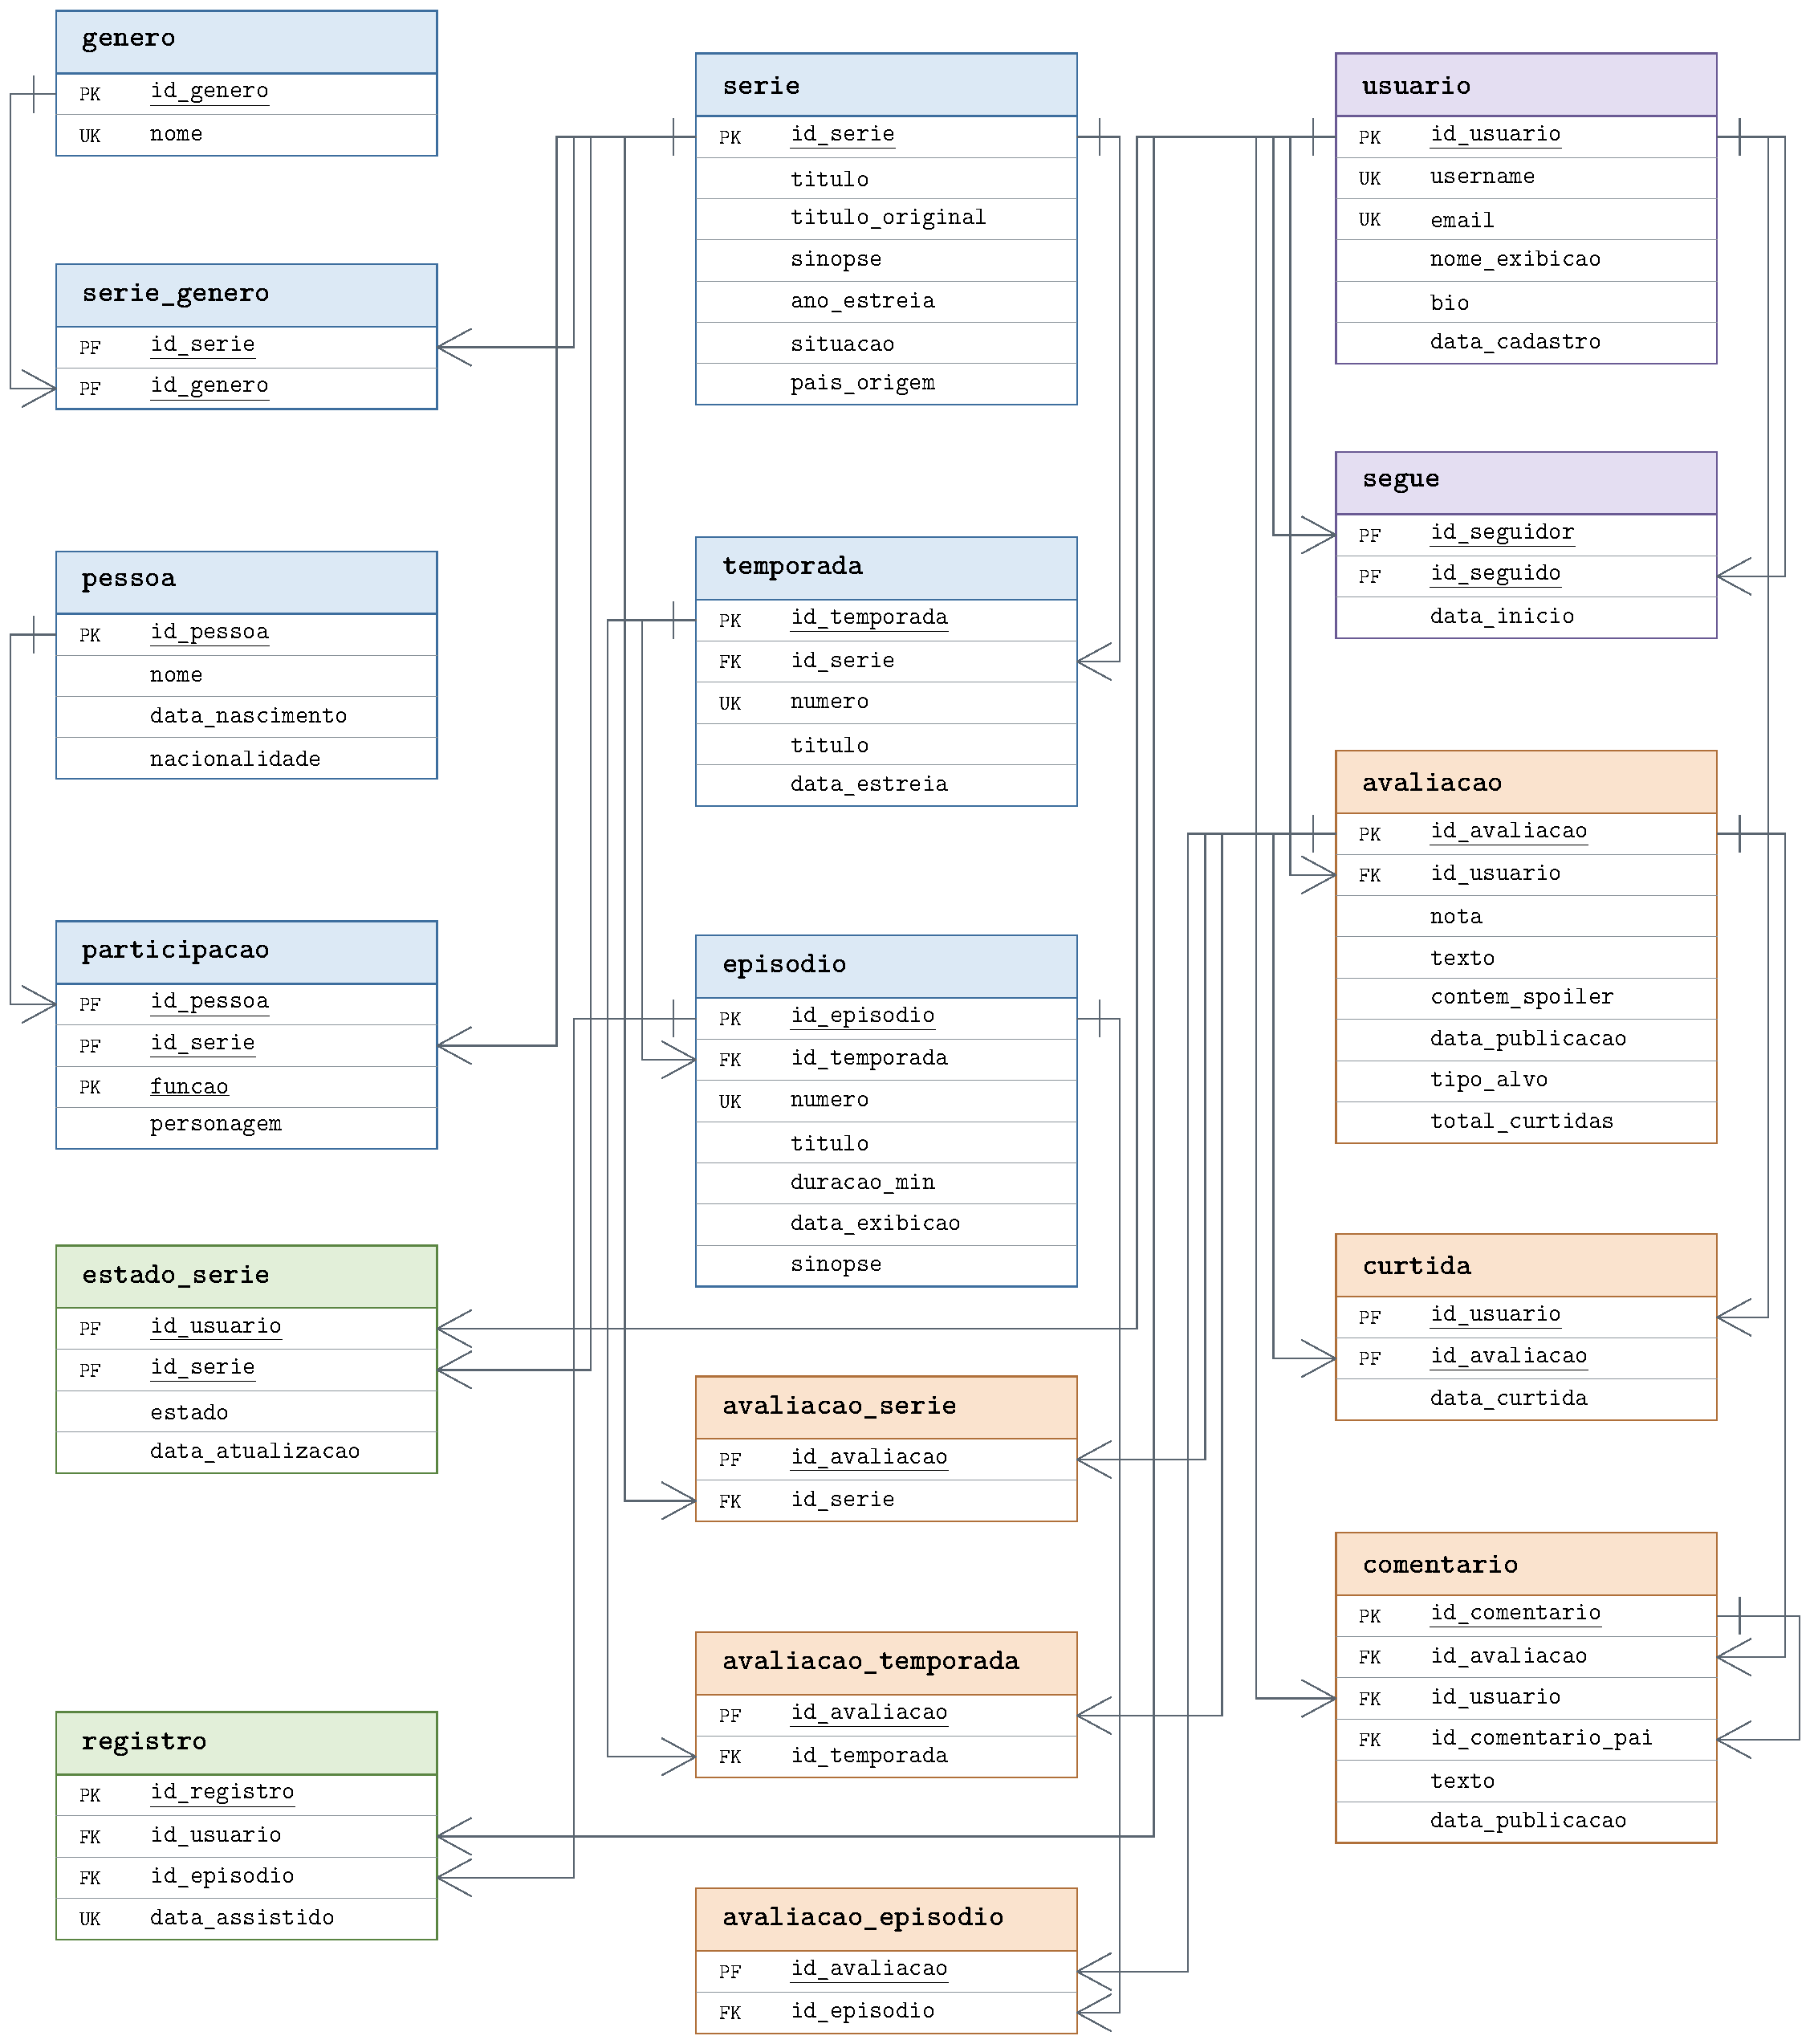
\includegraphics[width=\textwidth]{der-logico.png}
%     \caption{Diagrama lógico do banco de dados}
%     \label{fig:der-logico}
% \end{figure}

% ============================================================================
\chapter{Modelagem Física}\label{cap:fisica}
% ============================================================================

\orientacao{Capítulo a ser escrito. Contém o script SQL executável no PostgreSQL e
sua explicação. O script completo vai no apêndice ou em arquivo anexo; neste
capítulo entram os trechos que ilustram decisões, sempre acompanhados de
explicação. Código sem texto explicativo não pontua.}

\section{Convenções de nomenclatura e criação do esquema}

\orientacao{Registrem as convenções adotadas -- elas já estão em uso no
Capítulo~\ref{cap:conceitual} e devem ser seguidas: nomes de tabela no singular e
em minúsculas; chave primária no formato \id{id\_<tabela>}; \id{snake\_case} para
colunas compostas; objetos criados dentro de um esquema próprio, e não em
\id{public}.}

\begin{lstlisting}[caption={Criação do esquema},label={lst:schema}]
DROP SCHEMA IF EXISTS serie_tracker CASCADE;
CREATE SCHEMA serie_tracker;
SET search_path TO serie_tracker;
\end{lstlisting}

\section{Definição de dados (DDL)}

\orientacao{Apresentem os comandos \id{CREATE TABLE} na ordem correta de
dependência: uma tabela só pode ser criada depois daquelas que ela referencia. A
ordem da lista da Seção~\ref{sec:esquema-relacional} já respeita isso e pode ser
seguida diretamente. Não é necessário reproduzir as 17 tabelas no corpo do texto;
selecionem as mais representativas -- sugestão: \id{episodio} (entidade fraca com
\id{UNIQUE} sobre a chave parcial), \id{participacao} (chave composta e
\id{CHECK} cruzado entre colunas) e \id{avaliacao} com uma de suas subclasses
(especialização, em que a chave primária é também chave estrangeira).}

\section{Restrições de integridade}

\orientacao{Organizem por tipo, seguindo o item 5 do conteúdo programático, e
citem a regra de negócio correspondente ao lado de cada restrição:
\begin{itemize}[nosep]
    \item \textbf{Restrições de domínio} -- \id{NOT NULL}, \id{CHECK},
    \id{UNIQUE}. Casos a destacar: faixa e granularidade da nota (RN16);
    avaliação não vazia (RN17); data de exibição não futura (RN12);
    \id{funcao} e \id{personagem} coerentes entre si (RN10); proibição de
    seguir a si mesmo (RN03).
    \item \textbf{Integridade referencial} -- justifiquem a política de cada
    chave estrangeira. Use-se \id{ON DELETE CASCADE} onde há dependência
    existencial (RN04, RN08, RN24) e \id{ON DELETE RESTRICT} onde a exclusão
    deve ser impedida por representar perda de informação do acervo.
\end{itemize}}

\section{Gatilhos}\label{sec:gatilhos}

\orientacao{Cinco gatilhos estão previstos. Para cada um, apresentem o código e --
mais importante -- expliquem \textbf{por que um gatilho é necessário}, isto é, por
que uma restrição declarativa não resolveria. Esse é o argumento que diferencia um
trabalho bom de um trabalho apenas correto.}

\begin{table}[H]
\centering
\caption{Gatilhos a implementar}
\label{tab:gatilhos}
\small
\begin{tabularx}{\textwidth}{@{}llX@{}}
\toprule
\textbf{Gatilho} & \textbf{Evento} & \textbf{Regra garantida} \\
\midrule
\id{trg\_avaliacao\_exige\_registro} &
\textsc{before insert} em \id{avaliacao\_episodio} &
RN18 -- só se avalia episódio já registrado como assistido. Exige consulta a
outra tabela, o que um \id{CHECK} não pode fazer. \\
\addlinespace
\id{trg\_avaliacao\_unica\_por\_alvo} &
\textsc{before insert} nas três subclasses &
RN19 -- uma avaliação por usuário por alvo. O autor está na superclasse e o alvo
na subclasse, de modo que nenhuma restrição \id{UNIQUE} alcança as duas colunas
simultaneamente. \\
\addlinespace
\id{trg\_bloqueia\_autocurtida} &
\textsc{before insert} em \id{curtida} &
RN22 -- ninguém curte a própria avaliação. A comparação envolve uma coluna de
outra tabela. \\
\addlinespace
\id{trg\_atualiza\_contador\_curtidas} &
\textsc{after insert/delete} em \id{curtida} &
Mantém o atributo derivado \id{total\_curtidas} (Seção~\ref{sec:derivados})
sincronizado com a contagem real. \\
\addlinespace
\id{trg\_garante\_estado\_assistindo} &
\textsc{after insert} em \id{registro} &
RN14 -- registrar um episódio promove a série a \textit{assistindo}. Regra de
propagação de estado, inexprimível de forma declarativa. \\
\bottomrule
\end{tabularx}
\end{table}

\section{Visões}

\orientacao{Duas visões estão previstas (item 4.6 do conteúdo programático).
Apresentem o código e o problema que cada uma resolve.
\begin{itemize}[nosep]
    \item \id{vw\_avaliacao\_completa} -- reúne a superclasse e as três
    subclasses em um único conjunto de linhas, resolvendo o título do alvo
    (nome da série, identificação da temporada ou do episódio). Implementada com
    \id{UNION ALL}, exercita operações de conjunto e resolve, do lado da leitura,
    a fragmentação introduzida pela especialização. É a visão que as consultas da
    seção seguinte devem usar.
    \item \id{vw\_progresso\_serie} -- para cada par usuário-série, apresenta
    episódios distintos assistidos, total de episódios e percentual de progresso.
    Atenção: use-se \id{COUNT(DISTINCT id\_episodio)}, pois a RN11 permite
    registros repetidos do mesmo episódio e a contagem simples inflaria o
    progresso.
\end{itemize}}

\section{Carga de dados (DML)}

\orientacao{A carga precisa ser \textbf{coerente e suficiente}: coerente no
sentido de respeitar todas as restrições e gatilhos (por exemplo, não tente
inserir avaliação de episódio sem inserir antes o registro correspondente, ou a
carga falhará por causa da RN18); suficiente no sentido de permitir que as três
consultas da próxima seção retornem resultados não triviais.

Dimensionamento sugerido: 6 a 8 usuários, 5 a 6 séries com 2 a 3 temporadas cada,
6 a 10 episódios por temporada, 8 a 10 gêneros, 10 a 15 pessoas com participações
variadas, um grafo de seguidores com pelo menos um caso de relação não recíproca,
40 ou mais registros de exibição, 20 ou mais avaliações distribuídas entre os três
níveis, e curtidas e comentários suficientes para que a ordenação por popularidade
produza um ranking com empates desfeitos.

Ordem de inserção: a mesma da criação das tabelas. Insiram os registros de
exibição \emph{antes} das avaliações de episódio.}

\section{Consultas de exemplo}

\orientacao{Três consultas que demonstrem a utilidade do banco no minimundo. Para
cada uma: enunciem em português a pergunta respondida, apresentem o SQL, mostrem o
resultado obtido e comentem-no. As três abaixo foram escolhidas para cobrir itens
distintos do conteúdo programático -- não as substituam por variações do mesmo
tipo de consulta.}

\subsection{Consulta 1 -- Ranking de séries por nota média}

\orientacao{\textit{Quais séries têm as melhores avaliações entre os usuários,
considerando apenas as que receberam número significativo de notas?}

Exercita junção múltipla, funções agregadas (\id{AVG}, \id{COUNT}),
\id{GROUP BY} e \id{HAVING}. O \id{HAVING COUNT(*) >= 3} é o ponto central:
sem ele, uma série com uma única nota 5,0 lideraria o ranking, o que evidencia
por que a cláusula existe. Comentem isso.}

\subsection{Consulta 2 -- Atividade recente de quem o usuário segue}

\orientacao{\textit{Quais foram as últimas avaliações publicadas pelos usuários
que determinado usuário segue?}

Exercita subconsulta aninhada (\id{IN} ou \id{EXISTS} sobre \id{segue}),
auto-relacionamento e uso de visão (\id{vw\_avaliacao\_completa}). Vale apresentar
as duas formulações -- com \id{IN} e com \id{EXISTS} -- e comentar a diferença.}

\subsection{Consulta 3 -- Séries na lista de interesse ainda não iniciadas}

\orientacao{\textit{Quais séries o usuário marcou como ``pretendo assistir'' sem
ter assistido nenhum episódio até agora?}

Exercita operação de conjunto (\id{EXCEPT}), que é o item 4.3 do conteúdo. É a
consulta que sustenta a funcionalidade real de ``comece por aqui''. Vale mostrar
também a formulação equivalente com \id{NOT EXISTS} e comentar que ambas retornam
o mesmo conjunto.}

\section{Rastreabilidade das regras de negócio}\label{sec:rastreabilidade}

\orientacao{Tabela de fechamento do trabalho: para cada regra da
Seção~\ref{sec:regras}, indiquem onde ela foi implementada. Regras sem
implementação precisam ser justificadas -- normalmente porque pertencem à camada
da aplicação. Esta tabela é a melhor defesa possível numa arguição, porque mostra
que nada foi enunciado e esquecido.}

\begin{longtable}{@{}p{1.6cm}p{5.2cm}p{9cm}@{}}
\toprule
\textbf{Regra} & \textbf{Implementada por} & \textbf{Observações} \\
\midrule
\endhead
RN01 & & \\
RN02 & & \\
RN03 & & \\
RN04 & & \\
RN05 & & \\
RN06 & & \\
RN07 & & \\
RN08 & & \\
RN09 & & \\
RN10 & & \\
RN11 & & \\
RN12 & & \\
RN13 & & \\
RN14 & & \\
RN15 & & \\
RN16 & & \\
RN17 & & \\
RN18 & & \\
RN19 & & \\
RN20 & & \\
RN21 & & \\
RN22 & & \\
RN23 & & \\
RN24 & & \\
\bottomrule
\end{longtable}

\iforientacoes
% ============================================================================
\appendix
\chapter{Divisão de trabalho e convenções do grupo}
% ============================================================================

Este apêndice é material interno e não faz parte da entrega. Ele desaparece do PDF
quando \verb|\orientacoesfalse| é acionado.

\section{Atribuições}

\begin{table}[H]
\centering
\small
\begin{tabularx}{\textwidth}{@{}llX@{}}
\toprule
\textbf{Integrante} & \textbf{Parte} & \textbf{Entrega} \\
\midrule
Igor & Capítulo~\ref{cap:conceitual} &
Concluído: minimundo, 24 regras de negócio, dicionário de
dados, cardinalidades, especialização, agregação. Falta apenas desenhar o DER no
brModelo. \\
\addlinespace
-- & Capítulo~\ref{cap:logica} &
Mapeamento ER\,$\rightarrow$\,relacional, esquema relacional, dependências
funcionais, demonstração de normalização e diagrama lógico. \\
\addlinespace
-- & Capítulo~\ref{cap:fisica}, seções 1--5 &
DDL das 17 tabelas, restrições de integridade, os cinco gatilhos e as duas visões. \\
\addlinespace
-- & Capítulo~\ref{cap:fisica}, seções 6--8 &
Carga de dados, as três consultas com resultados comentados e a tabela de
rastreabilidade. Responsável também por executar o script inteiro do zero e
confirmar que roda sem erro. \\
\bottomrule
\end{tabularx}
\end{table}

\section{Contrato de nomes}

O Capítulo~\ref{cap:conceitual} é a fonte de verdade para nomes de tabelas,
colunas, tipos e domínios. Ninguém deve renomear nada durante a escrita dos
capítulos seguintes sem atualizar o capítulo conceitual na mesma edição. O erro
mais comum neste tipo de trabalho é o esquema físico divergir do diagrama
conceitual -- e ele é penalizado porque torna o documento internamente
contraditório.

Em caso de necessidade real de mudança, anunciem ao grupo antes de alterar.

\section{Verificação antes da entrega}

\begin{enumerate}[nosep]
    \item O script SQL executa do zero, em banco vazio, sem erro e sem
    advertência.
    \item Toda regra de negócio da Seção~\ref{sec:regras} aparece preenchida na
    tabela de rastreabilidade.
    \item Os nomes no DDL coincidem com os do dicionário de dados.
    \item As duas figuras de diagrama estão presentes e com os blocos
    descomentados.
    \item Os integrantes e RAs na capa estão corretos.
    \item \verb|\orientacoestrue| foi trocado por \verb|\orientacoesfalse|.
    \item O sumário foi regenerado (compilar duas vezes).
\end{enumerate}
\fi

\end{document}
